%
%===============>>  ГРУППА 5-1 МОДУЛЬ 7  <<=============
%
\setmodule{7}

%BEGIN_FOLD % ====>>_____ Занятие 1 _____<<====
\begin{class}[number=1]
	\begin{listofex}
		\item Выполните действия:
		\begin{tasks}(1)
			\task \( 11,47+(3,89-2,11)-4,416+3,711 \)
			\task \( 3,16+(7,84-4,181)-3,11+14,816 \)
			\task \( 1,49+(6,13-4,12)-0,5+7,289 \)
		\end{tasks}
		\item Вычислите:
		\begin{tasks}(4)
			\task \( 0,5\cdot10 \)
			\task \( 0,15\cdot10000 \)
			\task \( 50,265\cdot10 \)
			\task \( 21,598\cdot1000 \)
			\task \( 9,56\cdot50 \)
			\task \( 8,532\cdot1200 \)
			\task \( 9,123\cdot15000 \)
			\task \( 24,1\cdot130000 \)
		\end{tasks}
		\item Вычислите:
		\begin{tasks}(4)
			\task \( 25,36\cdot1,2 \)
			\task \( 3,5\cdot3,8 \)
			\task \( 63,25\cdot0,3 \)
			\task \( 5,369\cdot0,05 \)
			\task \( 12,03\cdot4,6 \)
			\task \( 23,71\cdot1,8 \)
			\task \( 0,24\cdot5,5 \)
			\task \( 0,7\cdot0,14 \)
		\end{tasks}
		\item Найдите:
		\begin{tasks}(2)
			\task \( 3,5\% \) от \( 1400 \)
			\task \( 12,5\% \) от \( 12500 \)
			\task \( 25,5\% \) от \( 14 \)
			\task \( 0,3\% \) от \( 2 \)
		\end{tasks}
		\item Цену на блузку понизили на \( 11,5\% \). Какой стала её цена, если первоначально она стоила \( 5000 \) рублей?
		\item Максим построил у себя в тетради прямоугольник со сторонами, равными \( 1,8 \) см и \( 5,6 \) см. Найдите периметр и площадь фигуры. Что больше? На сколько?
		\item Костя изобразил треугольник, один угол которого равен \( 23,5\degree \), другой в \( 3,7 \) раза больше. Чему равен третий угол? Чему равны внешние углы этого треугольника?
	\end{listofex}
\end{class}
%END_FOLD

%BEGIN_FOLD % ====>>_____ Занятие 2 _____<<====
\begin{class}[number=2]
	\begin{listofex}
		\item Вычислите 
		\begin{tasks}(4)
			\task \( 1,8\cdot5,5 \)
			\task \( 41,7\cdot6,05 \)
			\task \( 8,42\cdot9,9 \)
			\task \( 6,703\cdot2,45 \)
			\task \( 55,3\cdot3,81 \)
			\task \( 6,321\cdot7,8 \)
			\task \( 32,4\cdot103,5 \)
			\task \( 8,05\cdot8,05 \)
		\end{tasks}
	\item Выполните действия
	\begin{tasks}
		\task \( 4,735\cdot0,5+14,95\cdot1,3+2,121\cdot0,7 \)
		\task \( (0,578+2,172)\cdot(1,823+0,117)-1,711\cdot(0,418+1,382) \)
		\task \( 3,006-0,0417\cdot3-0,875\cdot0,4 \)
	\end{tasks}
	\item Ширина прямоугольника \( 5,15 \) см, а длина в \( 2 \) раза больше. Найдите площадь и периметр данного прямоугольника?
	\item Площадь прямоугольника \( 42 \) см\( ^{2} \), ширина его равна \( 6 \) см. Чему равна длина прямоугольника?
	\item 
	\begin{minipage}[t]{\bodywidth}
		Найдите угол \( \alpha \).
	\end{minipage}
	\hspace{0.02\linewidth}
	\begin{minipage}[t]{\picwidth}
		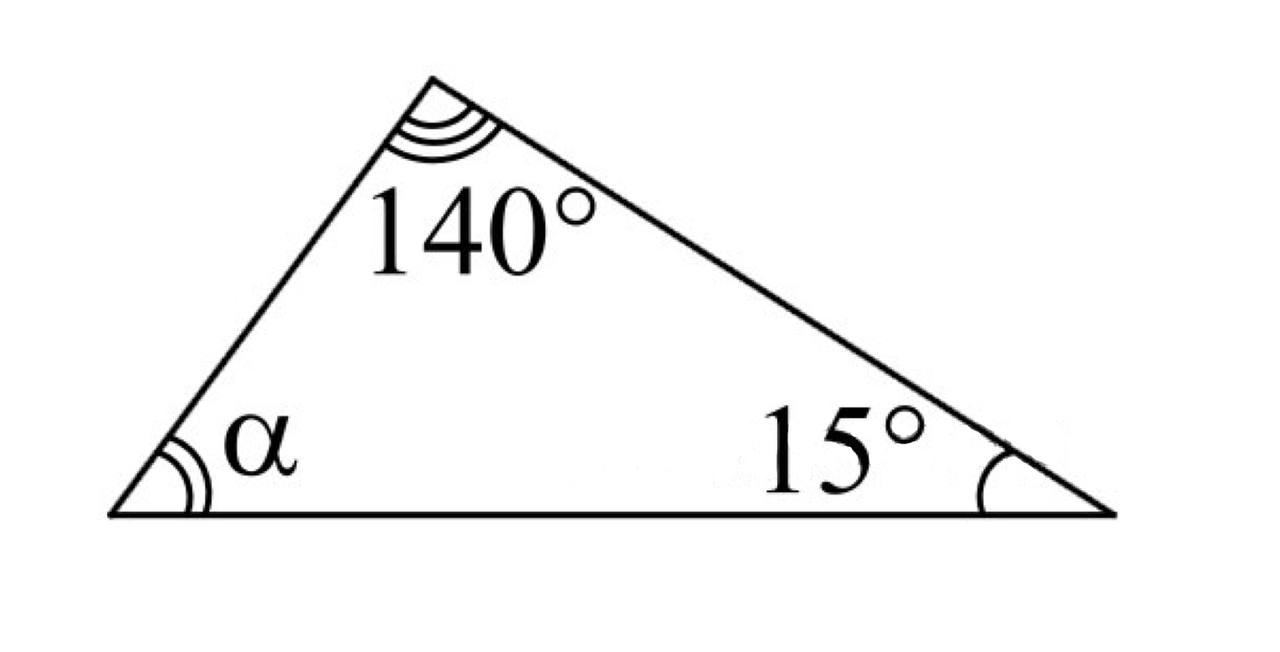
\includegraphics[align=t, width=\linewidth]{\picpath/G51M7L2-1}
	\end{minipage}
	\item 
	\begin{minipage}[t]{\bodywidth}
		Найдите величину угла \( MAB \).
	\end{minipage}
	\hspace{0.02\linewidth}
	\begin{minipage}[t]{\picwidth}
		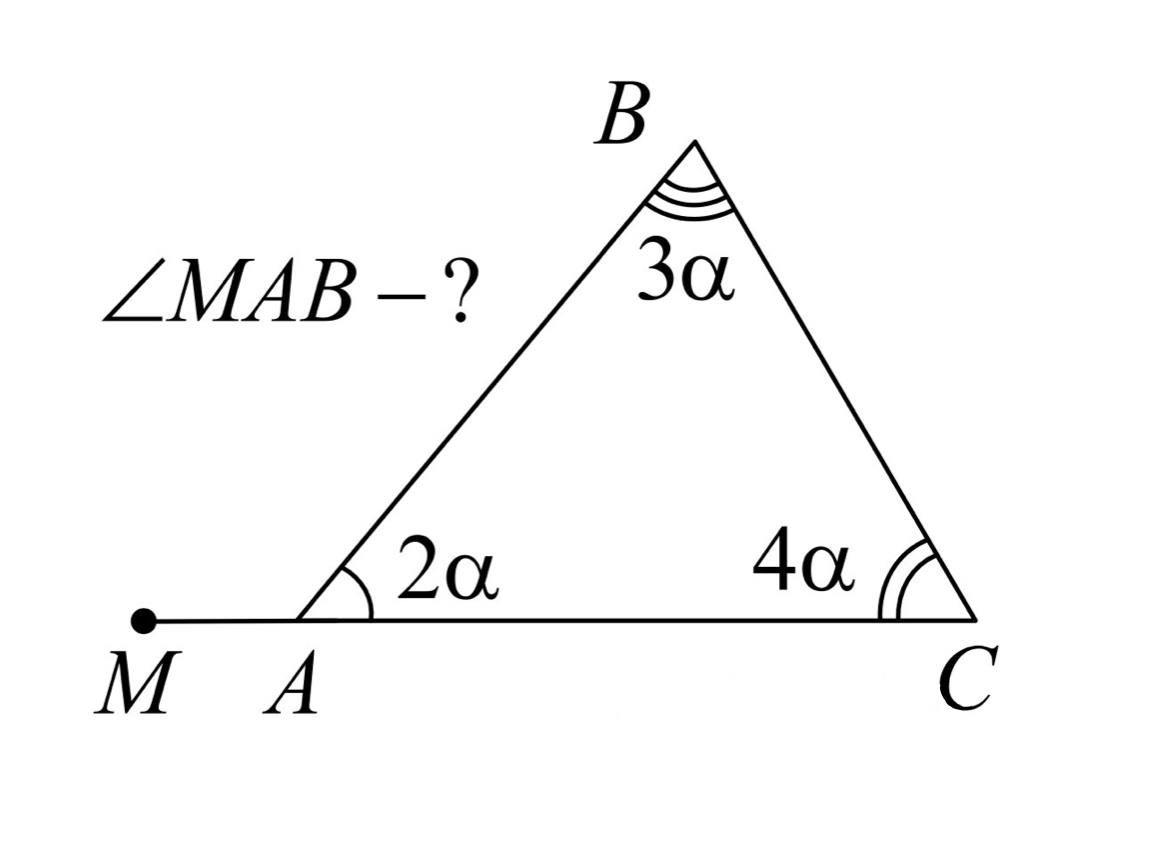
\includegraphics[align=t, width=\linewidth]{\picpath/G51M7L2-2}
	\end{minipage}
	\item Найдите углы треугольника, зная, что внешние углы при двух его вершинах равны \( 130^{\circ} \) и \( 140^{\circ} \).
	\item Один из углов, образовавшихся при пересечении двух прямых, равен \( 45^{\circ} \). Найди остальные углы.
	\item Биссектрисы углов \( N \) и \( M \) треугольника \(  MNP \) пересекаются в точке \( A \). Найдите \( \angle NAM \), если \( \angle N=84^{\circ} \) градусов , а \( \angle M=42 \)градусов . 
	\item Летом на дачу с детским садом собирались поехать \( 180 \) детей. Известно, что \( 15,4\% \) детей не поехали на дачу. Сколько всего детей в детском саду?
	\item Четверть тиража новой газеты раскуплена в первый же день ее выпуска, причем \( 64\% \) этой газеты продано в газетных киосках. Сколько процентов всего тиража продано в газетных киосках?
	\end{listofex}
\end{class}
%END_FOLD

%BEGIN_FOLD % ====>>_ Домашняя работа 1 _<<====
\begin{homework}[number=1]
	\begin{listofex}
		\item Вычислите:
		\begin{tasks}(2)
			\task \( 0,763-0,321+5,8 \)
			\task \( 10,5-6,957+11,87 \)
		\end{tasks}
		\item Вычислите 
		\begin{tasks}(4)
			\task \( 1,6\cdot10 \)
			\task \( 5,8\cdot100 \)
			\task \( 15,3\cdot200 \)
			\task \( 87,701\cdot 140 \)
		\end{tasks}
	\item Вычислите 
	\begin{tasks}(3)
		\task \( 440,8\cdot0,001 \)
		\task \( 79,22\cdot31,59 \)
		\task \( 84,102\cdot13,4 \)
	\end{tasks}
		\item Бассейн имеет форму прямоугольника со сторонами \( 5,32 \) м и \( 4,74 \) м. Чему равна его площадь?
		\item Все стороны семиугольника имеют длину \( 9,47 \) см. Найдите периметр фигуры.
	\end{listofex}
\end{homework}
%END_FOLD

%BEGIN_FOLD % ====>>_____ Занятие 3 _____<<====
\begin{class}[number=3]
	\begin{listofex}
		\item Выполните сложение: \begin{tasks}(3)
			\task \( 0,769 + 42,389; \)
			\task \( 5,8 + 22,191;  \)
			\task \( 95,381 + 3,219; \)
			\task \( 8,9021 + 0,68;  \)
			\task\(  2,7 + 1,35 + 0,8;  \)
			\task\( 13,75 + 8,2 + 0,115. \)
		\end{tasks}
		\item Выполните умножение:\begin{tasks}(3)
			\task \( \dfrac{3}{8}\cdot4,8 \)
			\task\( \dfrac{4}{25}\cdot3,45 \)
			\task\( \dfrac{9}{11}\cdot7,7 \)
			\task\( \dfrac{3}{16}\cdot9,6 \)
			\task\( \dfrac{15}{49}\cdot1,47 \)
			\task\( \dfrac{6}{9}\cdot0,54 \)
		\end{tasks}
		\item Выполните умножение:
		\begin{tasks}(3)
			\task \( \mfrac{1}{2}{9}\cdot0,81 \)
			\task \( \mfrac{7}{3}{4}\cdot2,4 \)
			\task \( \mfrac{4}{5}{28}\cdot 5,6 \)
			\task \( \mfrac{3}{9}{17} \cdot 6,8 \)
			\task \( \mfrac{7}{6}{7}\cdot 4,2 \)
			\task \( \mfrac{4}{5}{6}\cdot3,6 \)
		\end{tasks}
		\item Сторона квадрата \( \dfrac{7}{8} \) м. Чему равна площадь квадрата?
		\item У прямоугольного параллелепипеда высота равна \( 0,4 \) дм, длина \( \dfrac{3}{5} \) дм, и ширина \( 6,25 \) дм. Найдите его объем.
		\item Углы треугольника равны \( 63,21^{\circ} \) и \( 91,64^{\circ} \). Найдите третий угол треугольника.
		\item Найдите периметр равнобедренного треугольника, основание которого равно \( 17,25 \) см, а боковая сторона – \( 21,13 \) см.
		\item При пересечении двух прямых образовались углы. Один из углов равен \( 72,3\degree \). Чему равны остальные углы?
		\item Найдите периметр прямоугольника, если он составлен из трех квадратов: сторона одного из них \( 6,5 \) см, а сторона двух других по \( 3,25 \) см. 
		\item Ширина прямоугольника равна \( 5,2 \) см, а его длина на \( 2,15 \) см больше ширины. Периметр прямоугольника на \( 9,7 \) см больше периметра квадрата. Найдите сторону квадрата.
		\item Длина первого отрезка \( 12,9 \) см. Он в \( 3 \) раза длиннее, чем второй, а третий на \( 6,24 \) см короче, чем первый и второй вместе. Найдите длину каждого отрезка.
		\item Если сторону квадрата, периметр которого \( 36,9 \) см, уменьшить в 3 раза, то получится ширина прямоугольника, периметр которого \( 42,8 \) см. Найдите длину этого прямоугольника и вычислите его площадь.
	\end{listofex}
\end{class}
%END_FOLD

%BEGIN_FOLD % ====>>_____ Занятие 4 _____<<====
\begin{class}[number=4]
	\begin{listofex}
		\item Вычислите:
		\begin{tasks}(3)
			\task \( 53,5\cdot0,1 \)
			\task \( 45,6\cdot0,01 \)
			\task \( 292,8\cdot0,001 \)
			\task \( 98,23\cdot0,01 \)
			\task \( 801\cdot0,001 \)
			\task \( 44,4\cdot0,1 \)
		\end{tasks}
		\item Вычислите:
		\begin{tasks}(3)
			\task \( 66,103:100 \)
			\task \( 123,2:100 \)
			\task \( 493,3:1000 \)
			\task \( 53235,03:10000 \)
			\task \( 23:100 \)
			\task \( 1944,9039:10 \)
		\end{tasks}
		\item Вычислите:
		\begin{tasks}(3)
			\task \( 1,75:0,001 \)
			\task \( 0,48:0,1 \)
			\task \( 86,75:0,1\)
			\task \( 20,7:0,01 \)
			\task \( 243,2:0,001 \)
			\task \( 88,298:0,0001 \)
		\end{tasks}
		\item Сумма двух чисел равна \( 1,9 \), а их разность равна \( 1,27 \). Найдите эти числа.
		\item Периметр квадрата равен \( 17,2 \). Найдите его сторону и площадь.
		\item Периметр треугольника равен \( 72,9 \), а его стороны относятся как \( 2:3:4 \). Найдите длины его сторон.
		\item В равнобедренном треугольнике основание в \( 2 \) раза меньше боковой стороны. Периметр этого треугольника равен \( 65,25 \). Найдите длины его сторон.
		\item Угол \( A \) треугольника \( ABC \) равен \( 123,9^{\circ} \), а угол \( B \) в \( 3 \) раза меньше угла \( A \). Найдите неизвестные углы.
		\item Внешний угол равнобедренного треугольника в 7 раз меньше внутреннего. Найдите все углы треугольника.
		\item Площадь прямоугольника равна \( 37,8 \) см\( ^{2} \), а длина равна \( 9 \) см. Найдите ширину и периметр данного прямоугольника.
		\item В двух коробках \( 7,8 \) кг конфет. Когда из одной коробки взяли \( 1,25 \) кг конфет, то в обеих коробках конфет стало поровну.Сколько конфет было в каждой коробке?
		\item Измерения прямоугольного параллелепипеда \( 5,2 \) см; \( 3,4 \) см и \( 2,6 \) см. Найдите общую длину всех рёбер прямоугольного параллелепипеда, сумму площадей всех его граней и его объём.
	\end{listofex}
\end{class}
%END_FOLD

%BEGIN_FOLD % ====>>_ Домашняя работа 2 _<<====
\begin{homework}[number=2]
	\begin{listofex}
		\item Выполните умножение:
		\begin{tasks}(3)
			\task \( \dfrac{4}{14}\cdot4,2 \)
			\task\( \dfrac{3}{10}\cdot4,5 \)
			\task\( \dfrac{5}{12}\cdot1,44 \)
			\task \( \mfrac{4}{6}{13}\cdot5,2 \)
			\task \( \mfrac{11}{6}{7}\cdot6,3 \)
			\task \( \mfrac{2}{13}{42}\cdot 8,4 \)
		\end{tasks}
		\item Вычислите: \begin{tasks}(3)
			\task \( 0,65\cdot0,1 \)
			\task \( 4,2031\cdot0,01 \)
			\task \( 333,003\cdot0,001 \)
			\task \( 98,21:1000 \)
			\task \( 3215,005:10000 \)
			\task \( 84,9:100 \)
		\end{tasks}
		\item Найдите периметр равнобедренного треугольника, основание которого равно \( 23,02 \) см, а боковая сторона – \( 45,153 \) см.
		\item Углы треугольника равны \( 43,467^{\circ} \) и \( 77,777^{\circ} \). Найдите третий угол треугольника.
		\item Угол \( A \) треугольника \( ABC \) равен \( 94,64^{\circ} \), а угол \( B \) в \( 5 \) раз меньше угла \( A \). Найдите неизвестные углы.
		\item Ширина прямоугольника равна \( 43,01 \) см, а длина равна \( 3,9 \) см. Площадь и периметр данного прямоугольника.
	\end{listofex}
\end{homework}
%END_FOLD

%BEGIN_FOLD % ====>>_____ Занятие 5 _____<<====
\begin{class}[number=5]
	\begin{listofex}
		\item Занятие 5
	\end{listofex}
\end{class}
%END_FOLD

%BEGIN_FOLD % ====>>_____ Занятие 6 _____<<====
\begin{class}[number=6]
	\begin{listofex}
		\item Занятие 6
	\end{listofex}
\end{class}
%END_FOLD

%BEGIN_FOLD % ====>>_ Домашняя работа 3 _<<====
\begin{homework}[number=3]
	\begin{listofex}
		\item Домашняя работа 3
	\end{listofex}
\end{homework}
%END_FOLD

%BEGIN_FOLD % ====>>_____ Занятие 7 _____<<====
\begin{class}[number=7]
	\title{Подготовка к проверочной}
	\begin{listofex}
		\item Занятие 7
	\end{listofex}
\end{class}
%END_FOLD

=%BEGIN_FOLD % ====>>_ Проверочная работа _<<====
\begin{exam}
	\begin{listofex}
		\item Проверочная
	\end{listofex}
\end{exam}
%END_FOLD